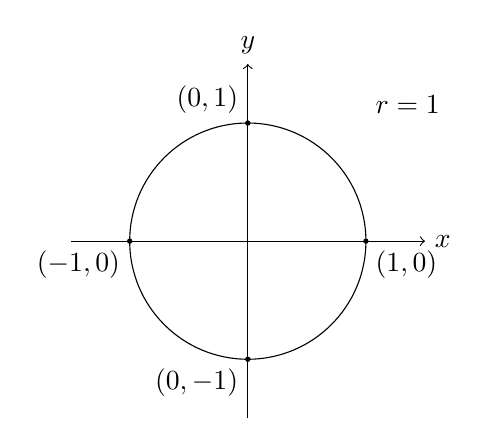
\begin{tikzpicture}[scale=1.5]
    \draw[->] (-1.5, 0) -- (1.5, 0) node [right] {\(x\)};
    \draw[->] (0, -1.5) -- (0, 1.5) node [above] {\(y\)};

    \draw (0, 0) circle (1) node at (1, 1) [above right] {\(r = 1\)};

    \draw[fill=black] (1, 0) circle (0.5pt) node [below right] {\((1, 0)\)};
    \draw[fill=black] (-1, 0) circle (0.5pt) node [below left] {\((-1, 0)\)};
    \draw[fill=black] (0, 1) circle (0.5pt) node [above left] {\((0, 1)\)};
    \draw[fill=black] (0, -1) circle (0.5pt) node [below left] {\((0, -1)\)};
\end{tikzpicture}